\documentclass[gray]{beamer}
\usepackage[utf8]{inputenc}
\usepackage[T2A]{fontenc}
\usepackage[english,russian]{babel}
% \usepackage{newtxtext,newtxmath}
\usepackage{lmodern}

\usepackage{graphicx} % Пакет для работы с изображениями
\usepackage{adjustbox} % Hyperlinks
\usepackage{courier}
\usepackage{blindtext}

\usepackage{float}
\usepackage{listings}

\usepackage{ragged2e}
\justifying

% \definecolor{c}{HTML}{000050}

% \usetheme{default}

\setbeamertemplate{footline}
{
  \leavevmode%
  \hbox{%
    \begin{beamercolorbox}[wd=\paperwidth,ht=2.5ex,dp=1.125ex,right]{page number in head/foot}%
      \usebeamerfont{page number in head/foot}\insertframenumber{} / \inserttotalframenumber\hspace{2ex}
    \end{beamercolorbox}%
  }
}

\setbeamertemplate{footline}[frame number]
\setbeamertemplate{navigation symbols}{}

\makeatletter
\setbeamertemplate{frametitle}{
  \begin{centering}
    \insertframetitle
    \par
  \end{centering}
}
\makeatother

\begin{document}

\begingroup
\setbeamertemplate{footline}{}
\begin{frame}
    \begin{minipage}{0.1\textwidth}
            \vspace{-0.1cm}
        
\includegraphics[width=1.5cm]{img/bmstu.pdf}
    \end{minipage}
    \hfill
    \begin{minipage}{0.8\textwidth}\centering\bfseries
        {
            \linespread{1}\selectfont\tiny
            \vspace{0.1cm}
            \textbf{Министерство~науки~и~высшего~образования~Российской~Федерации}

            \textbf{Федеральное~государственное~автономное~образовательное~учреждение высшего~образования}

            \textbf{<<Московский~государственный~технический~университет}

            \textbf{имени~Н.Э.~Баумана}

            \textbf{(национальный~исследовательский~университет)>>}

            \vspace{-0.2cm}
            \textbf{(МГТУ им. Н.Э.~Баумана)}
            \vspace{0.1cm}
        }
    \end{minipage}

    \vfill

    \begin{center}
    \Large Метод выделения составных частей научного текста на основе анализа распределения пикселей в сканирующей строке
    \end{center}

    \vfill

    Студент: Рунов Константин Алексеевич, ИУ7-84Б

    Научный руководитель: Строганов Юрий Владимирович

    \vfill

    \begin{center}
        \the\year\ г.
    \end{center}
\end{frame}
\endgroup

\begin{frame}
    \frametitle{Область применения}

    Для задач нормоконтроля требуется выделять составные части текстов, такие как текст, таблицы, листинги, рисунки, графики, схемы.
    
    \vfill

    Стандарт МГТУ для проведения нормоконтроля составляет~40 страниц за 8 часов.

    \vfill

    Количество документов, требующих обработки, постоянно увеличивается.
\end{frame}

\begin{frame}
    \frametitle{Цель и задачи}
    Целью работы является разработка метода для автоматического выделения составных частей научного текста, использующего только простые эвристики для классификации сегментов документа.
    % Цель работы. Ни в коем случае не должна повторять название. Мы должны расшифровать, каким образом будем ... + слова, связанные с разработкой программного продукта — это одно предложение.

    Задачи:
    \begin{itemize}
        \item Рассмотреть и сравнить существующие методы сегментации документов;
        \item Формализовать постановку задачи;
        \item Разработать описанный метод;
        \item Разработать программное обеспечение, реализующее данный метод;
        \item Исследовать скорость разметки и максимального объема используемой памяти в зависимости от количества процессов, участвующих в разметке.
    \end{itemize}
    
    % Основные задачи, которые мы решаем. Анализ предметной области с точки зрения формализации. Формализация сложного объекта и наличия ПО, поддерживающие данные и существующие методы — так прямо полностью и прописывать, плюсы, минусы.
\end{frame}

\begin{frame}
    \frametitle{Типы макетов документов}

\begin{figure}[H]
	\centering
    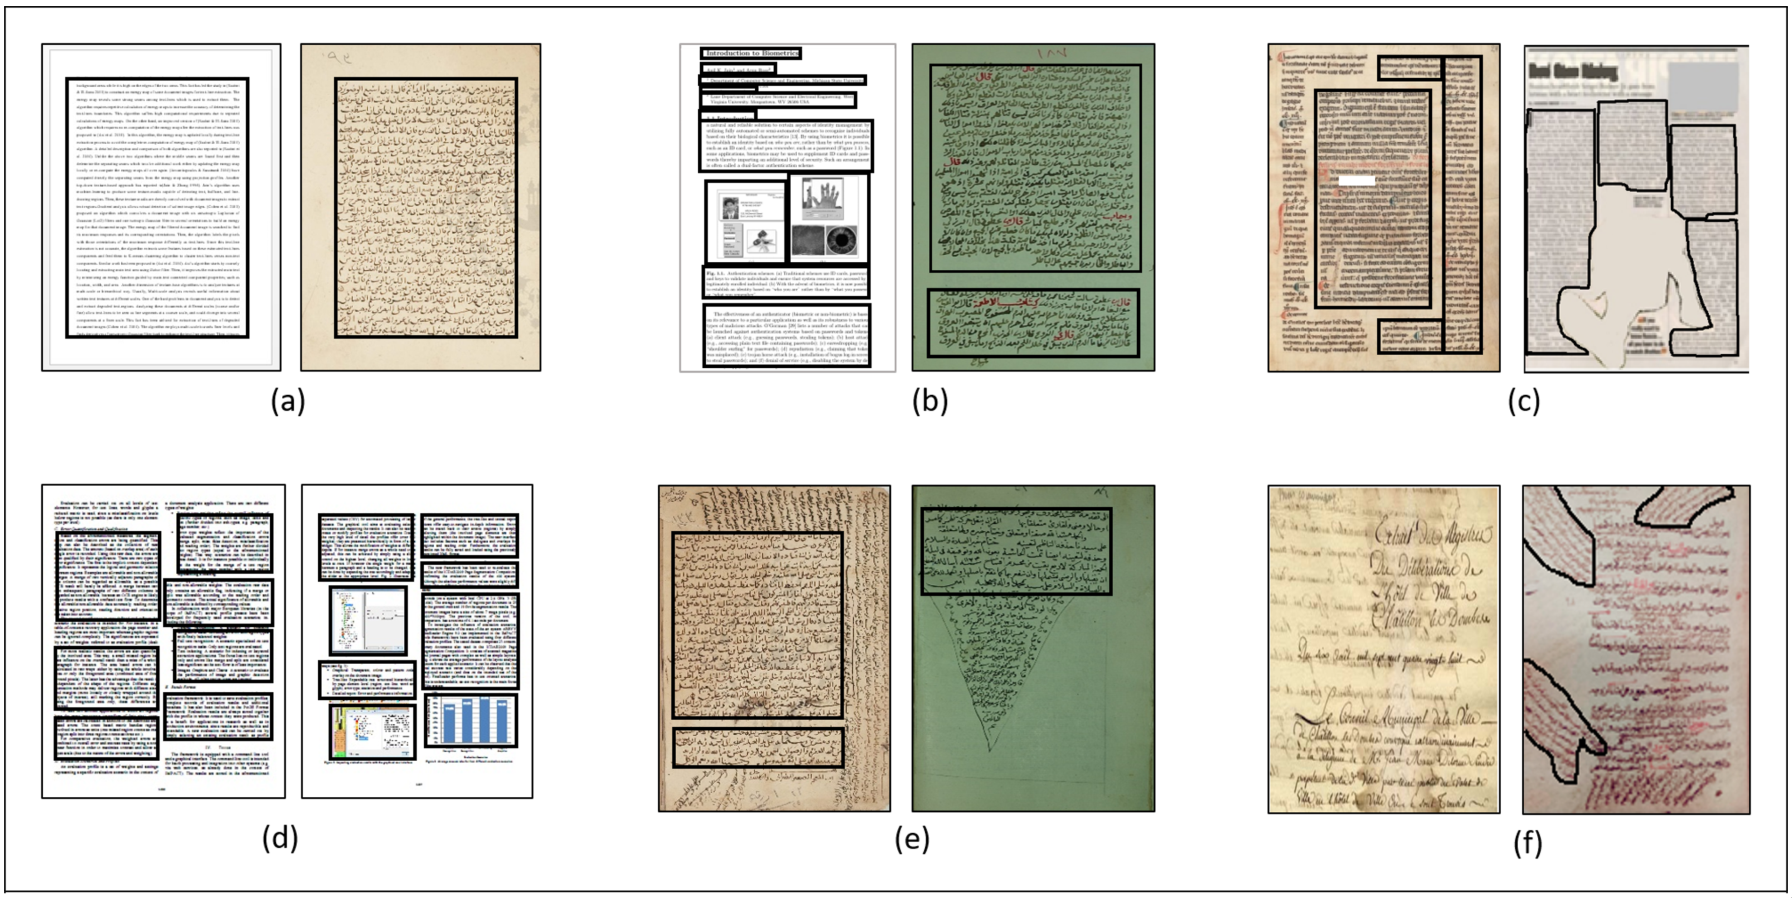
\includegraphics[width=\textwidth]{img/layouts.png}
\end{figure}

    Макеты документов: (a) Стандартный (прямоугольный), (b) Манхэттенский, (c) Не-Манхэттенский, (d) Многоколоночный Манхэттенский, (e) Произвольный (сложный), (f) С горизонтальным и диагональным наложением.

\end{frame}


\begin{frame}
    \frametitle{Классификация существующих методов сегментации}
    % Классификация методов, ПО. На нем будет много-много квадратиков (больше одного). Совершенно четко указывается наше место среди того, что разработано на данный момент. Мы занимаемся только маленьким левым нижним прямоугольничком.

    \begin{table}[H]
        % \centering
        \begin{center}
            \begin{tabular}{|c|c|c|c|c|}
                \hline
                \textbf{Метод \textbackslash\ Критерий} & \textbf{Скорость} & \textbf{Гибк.} & \textbf{Уст-ть} & \textbf{СпецТреб} \\ \hline
                % Connected Components Analysis        & 2 & 2 & 3 & Нет \\ \hline
                % Projection Profile Analysis        & 2 & 3 & 3 & Нет \\ \hline
                % Run-Length Smearing Algorithm       & 1 & 3 & 3 & Нет \\ \hline
                % Machine Learning Based         & 3 & 1 & 1 & Да \\ \hline
                % PPA + CCA  & 2 & 3 & 2 & Нет \\ \hline
                % Разраб. метод    & 1 & 3 & 3 & Да \\ \hline
                Con. Comp. An.        & 2 & 2 & 3 & Нет \\ \hline
                Proj. Prof. An.        & 2 & 3 & 3 & Нет \\ \hline
                Run-Len. Sm. Alg. & 1 & 3 & 3 & Нет \\ \hline
                Machine Learning         & 3 & 1 & 1 & Да \\ \hline
                PPA + CCA  & 2 & 3 & 2 & Нет \\ \hline
                Разраб. метод    & 1 & 3 & 3 & Да \\ \hline
            \end{tabular}
        \end{center}
    \end{table}

    % \raggedright

    % Скорость --- время, необходимое методу для обработки документа и получения результата разметки.
    %
    % \vspace{0.1cm}
    %
    Гибкость --- способность метода адаптироваться к различным типам макетов документов;

    \vspace{0.2cm}

    Устойчивость --- способность метода адаптироваться к шумам и искажениям текста;

    \vspace{0.2cm}

    Специальное требование --- позволяет сегментировать не только текст, но другие его составные части.
\end{frame}

\begin{frame}
    \frametitle{Формализация задачи}
    % Приложить математический аппарат к тому, что мы будем исследовать.

    Документ $ D = \{ P_1, P_2, \dots, P_n \} $ состоит из страниц $ P_1, \dots, P_n $, а каждая страница $ P_i $ состоит из множества сегментов $ S_{i,1}, \dots, $ $S_{i,m} $.

    \vspace{0.2cm}

    Сегмент $S_{i,j}$ --- кортеж $(x_{i,j}, y_{i,j}, w_{i,j}, h_{i,j})$, где $(x_{i,j}, y_{i,j})$ --- координаты верхнего левого угла, $w_{i,j}$ --- ширина, $h_{i,j}$ --- высота сегмента.

    \vspace{0.2cm}

    Требуется построить отображение
    $$
        F : D \to \{(S_{i,j}, C_{i,j})\},
    $$
    где каждому сегменту $S_{i,j}$ ставится в соответствие класс
    $$
        C_{i,j} = C_{i,j}(S_{i,j}),
    $$
    область допустимых значений которого определяется согласно требованиям к разметке.
\end{frame}



\begin{frame}
    \frametitle{Предлагаемый метод}
    % IDEF0 диаграмма. Четко объясняем комиссии, что на входе, что на выходе. Это сложно. A0 ограничиться нельзя — хотя бы A1.
    \begin{figure}[H]
        \begin{center}
            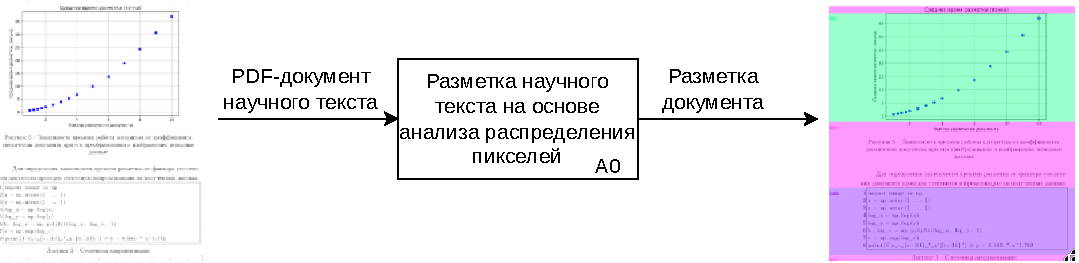
\includegraphics[width=\textwidth]{diag/a0-final.pdf}
        \end{center}
    \end{figure}

    % Кроме формул, перед ними, перед классификацией — четко показать, как входные данные преобразуются в выходные — IDEF0. После чего — классификация, формализация, математика.
\end{frame}

\begin{frame}
    \frametitle{Предлагаемый метод, детализация}
    \begin{figure}[H]
        \begin{center}
            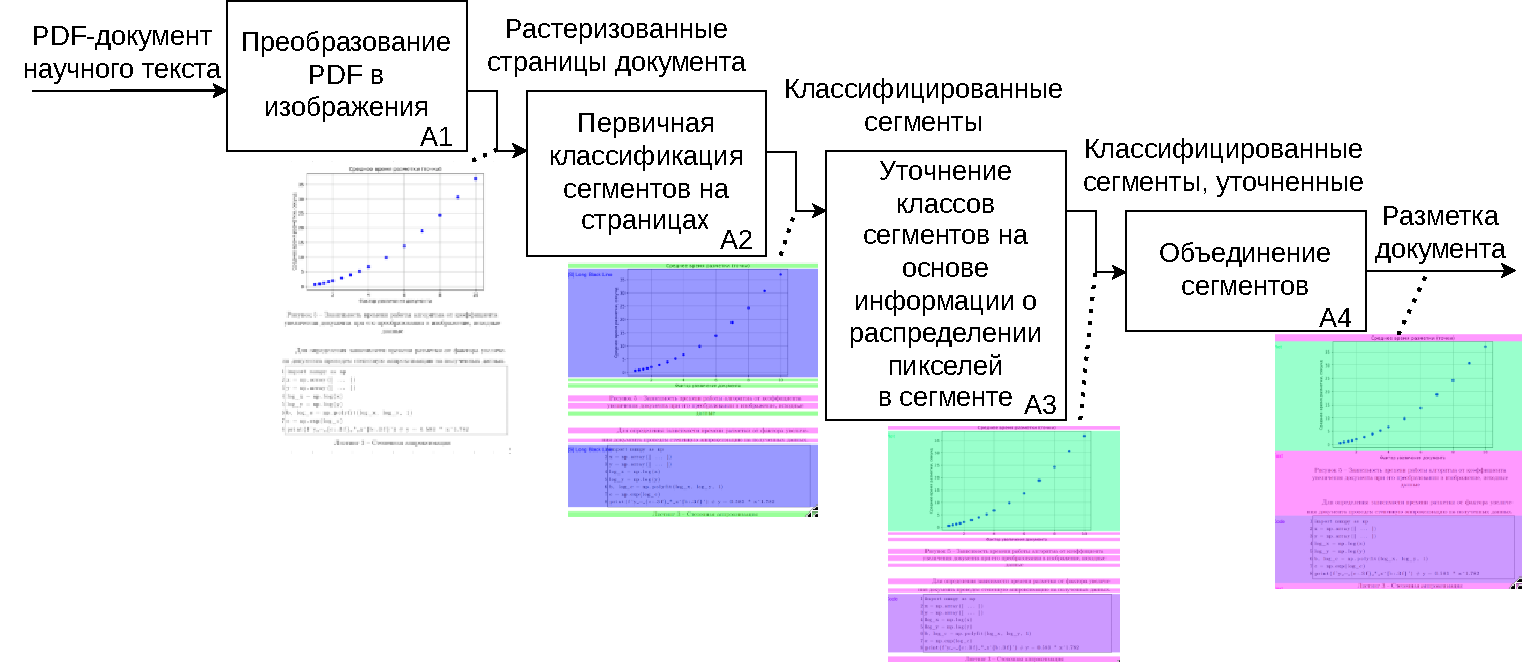
\includegraphics[width=\textwidth]{diag/a1-final.pdf}
        \end{center}
    \end{figure}
\end{frame}

\begin{frame}
    \frametitle{Предлагаемый метод, детализация первичной разметки}
    \begin{figure}[H]
        \begin{center}
            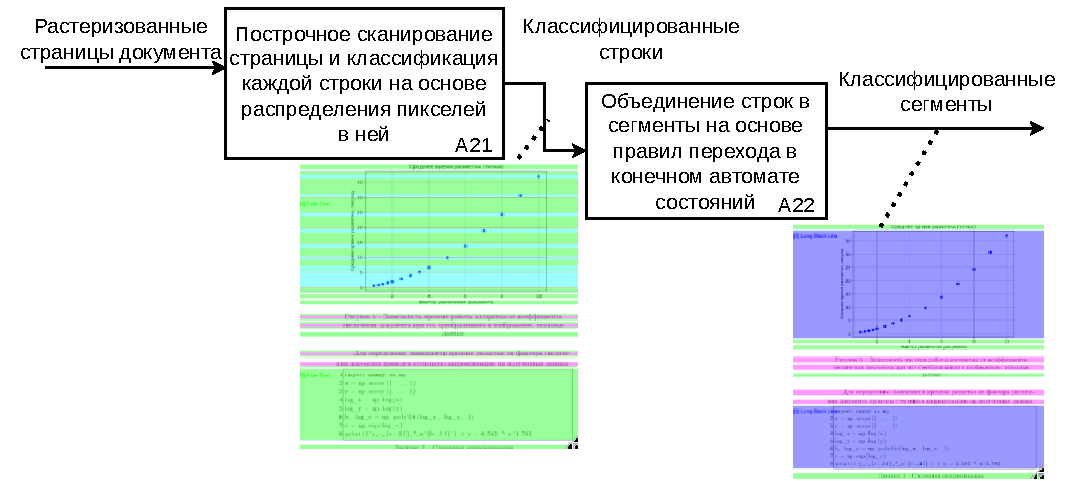
\includegraphics[width=\textwidth]{diag/a2-final.pdf}
        \end{center}
    \end{figure}
\end{frame}

\begin{frame}
    \frametitle{Первичная разметка}
    % 7-8 слайд «Разработка алгоритма». На презентации — в виде схемы алгоритма. Вербальное описание смотрится плохо. Рассказывать только особенности алгоритма, как он отличается от других

    \begin{figure}[H]
        \centering
        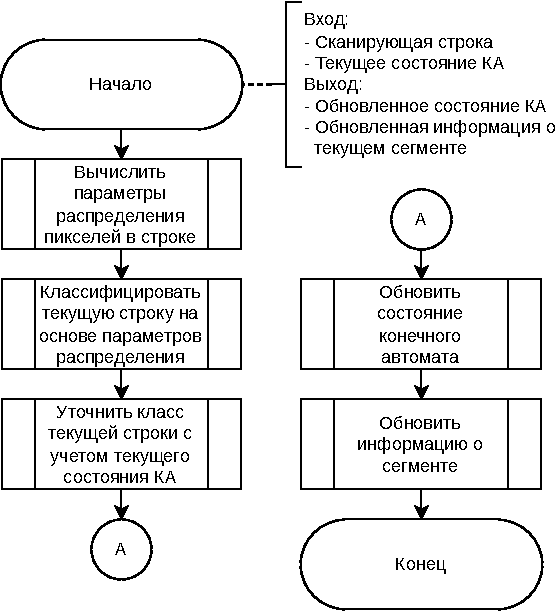
\includegraphics[width=0.7\textwidth]{diag/pres-primary.pdf}
    \end{figure}
\end{frame}

\begin{frame}
    \frametitle{Конечный автомат состояний сканирующей строки при первичной разметке}
    \begin{figure}[H]
        \centering
        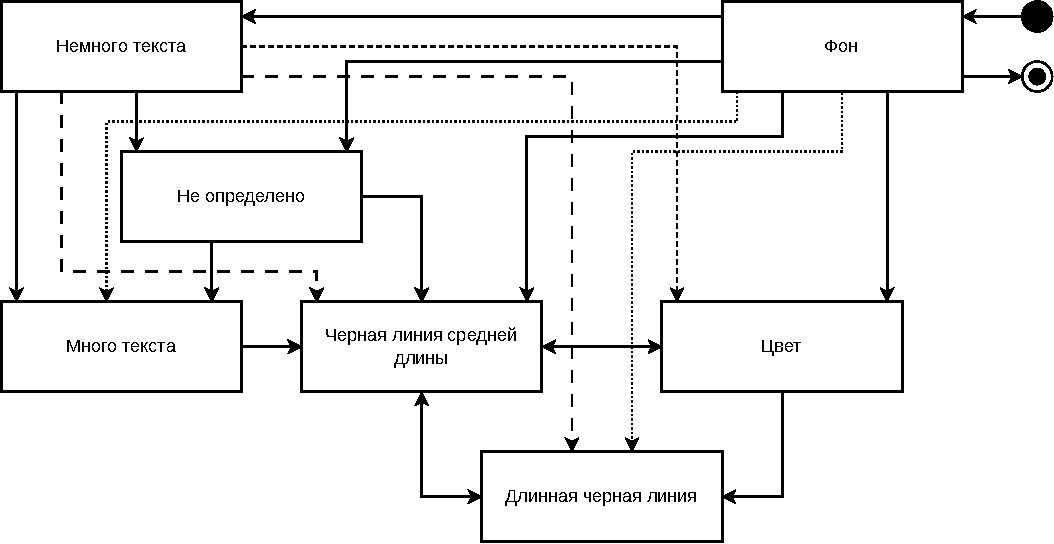
\includegraphics[width=\textwidth]{diag/fsm.full.pdf}
    \end{figure}
\end{frame}

\begin{frame}
    \frametitle{Первичная разметка. Примеры правил}
    Классификация сканирующей строки:
    \begin{itemize}
        \item Если в сканирующей строке \underline{большое} количество комнонент из смежных черных пикселей, строка относится к классу <<Много текста>>;
        \item Если сканирующая строка содержит цветные пиксели, она относится к классу <<Цвет>>;
        \item Если сканирующая строка содержит единственную компоненту из смежных черных пикселей длиной почти во всю ширину документа, она относится к классу <<Длинная черная линия>>.
    \end{itemize}

    Обновление состояния конечного автомата:
    \begin{itemize}
        \item Если КА находится в состоянии <<Фон>> и встречает строку, содержащую черные пиксели, и их распределение не похоже ни на текст, ни на черные линии, КА переходит в состояние <<Не определено>>.
    \end{itemize}
\end{frame}

\begin{frame}
    \frametitle{Алгоритм уточненной разметки}
    \begin{figure}[H]
        \centering
        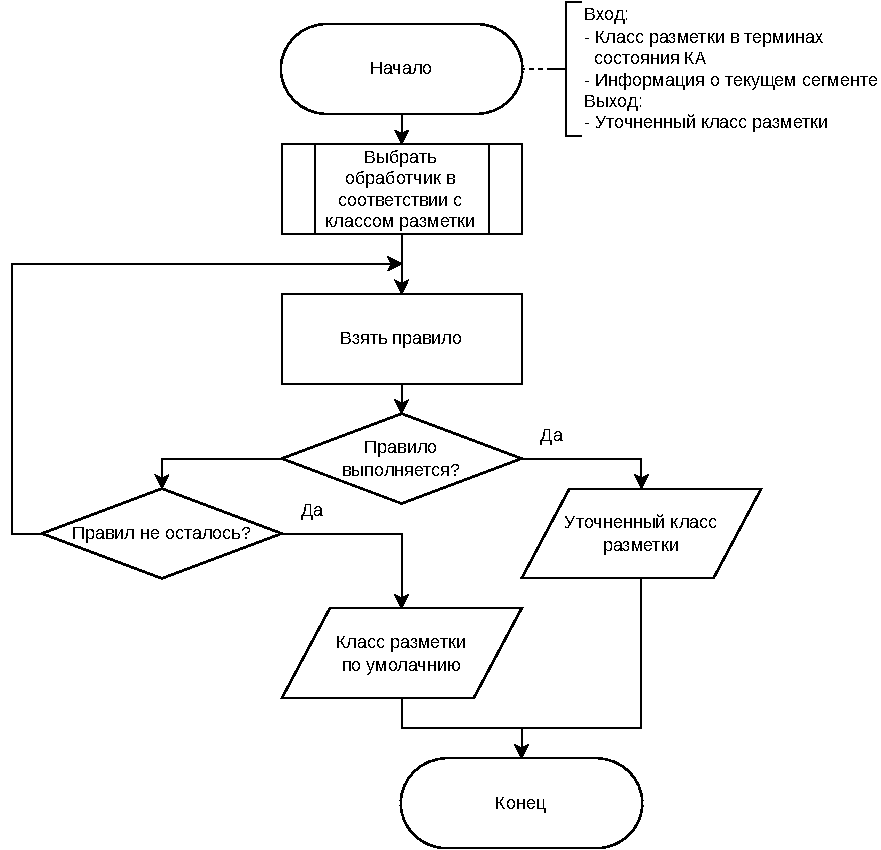
\includegraphics[width=0.8\textwidth]{diag/specified.pdf}
    \end{figure}
\end{frame}

\begin{frame}
    \frametitle{Уточненная разметка. Примеры правил}
    \begin{itemize}
        \item Если сегмент был классифицирован, как <<Не~определено>>, при этом его высота небольшая ИЛИ много строк в сегменте было классифицировано, как <<Немного~текста>>, то уточненный класс сегмента будет <<Текст>>;
        % \item Если сегмент был классифицирован, как <<Немного текста>>, то его уточненный класс --- <<Текст>>;
        \item Если сегмент был классифицирован, как <<Много~текста>>, но при этом из информации о сегменте видно, что в нем содержится больше двух столбцов черных пикселей высотой с сегмент, то его уточненный класс <<Таблица>>;
        \item Если сегмент был классифицирован, как <<Цвет>>, и содержит одну вертикальную линию, а также количество белых пикселей в сегменте преобладает, то его уточненный класс <<График>>.
    \end{itemize}
\end{frame}

\begin{frame}
    \frametitle{Алгоритм объединения сегментов}
    \begin{figure}[H]
        \centering
        \hspace{1cm}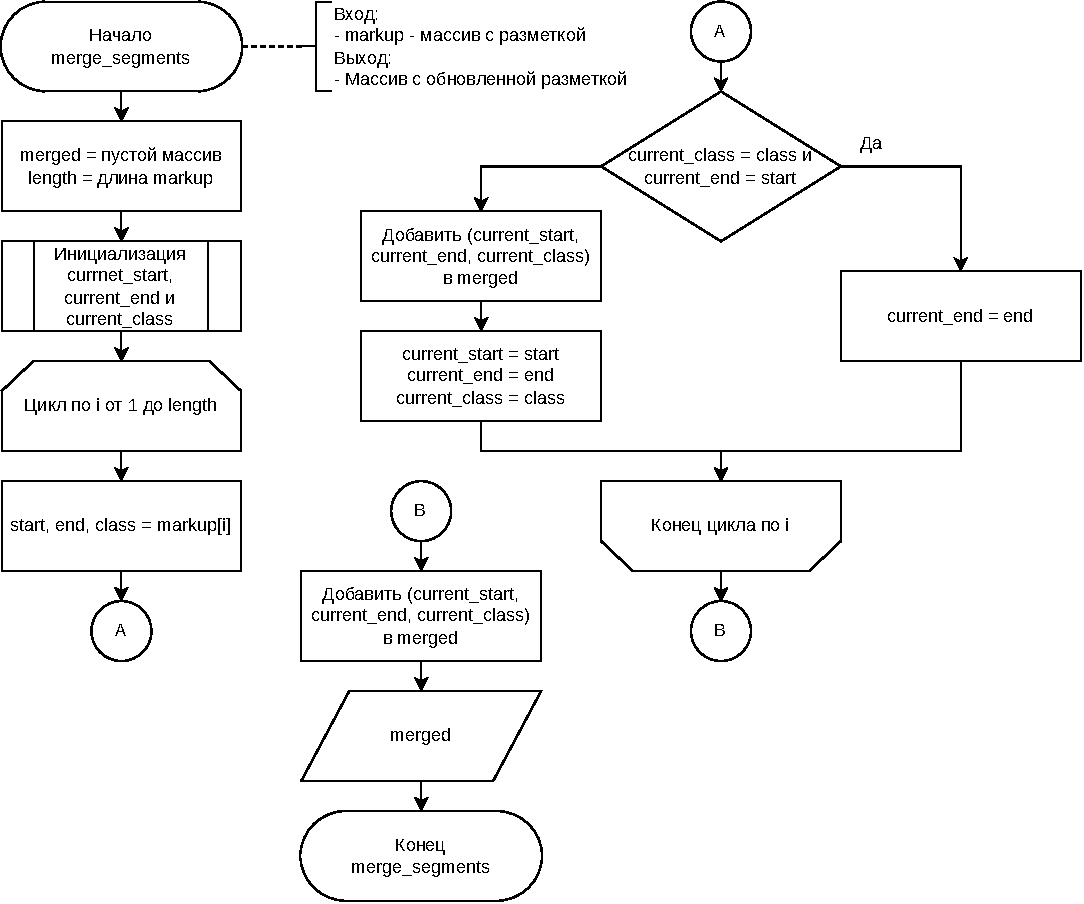
\includegraphics[width=0.9\textwidth]{diag/pres-merge.pdf}
    \end{figure}
\end{frame}

\begin{frame}
    \frametitle{Объединенная разметка. Примеры правил}
    \begin{itemize}
        \item Маленькие (меньше 30 пикселей) фоновые сегменты сливаются с наибольшим соседним;
        \item Фоновые сегменты сливаются с соседними, если у соседей одинаковый класс;
        \item Небольшие (меньше 200 пикселей) фоновые сегменты меняют класс на <<Не определено>>;
        \item Небольшие (меньше 200 пикселей) неопределенные сегменты сливаются с наибольшим соседним.
    \end{itemize}
\end{frame}

\begin{frame}
    \frametitle{Структура ПО}
    % Далее (9 слайд) — структура разрабатываемого ПО. Минимум — опуститься до модулей — что и как делали.
    \begin{figure}[H]
        \centering
        \hspace{-1.5cm}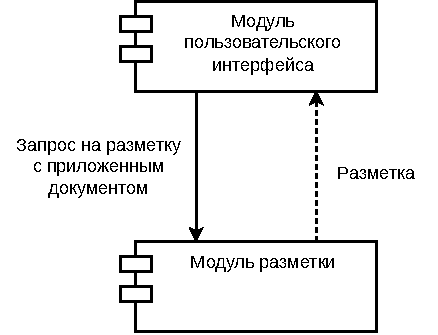
\includegraphics[width=0.9\textwidth]{diag/components.pdf}
    \end{figure}
\end{frame}

\begin{frame}
    \frametitle{Зависимость времени разметки от количества рабочих процессов}
    % Закончили основную часть, пришли к исследованию (10-11, минимум 2 слайда). Нельзя описать исследование и повторить заголовок. Только конкретика исследования. Если удастся создать что-то, что сравнимо с уже существующим — можно сравнить и по сложности, и по времени.
    \begin{figure}[H]
        \centering
        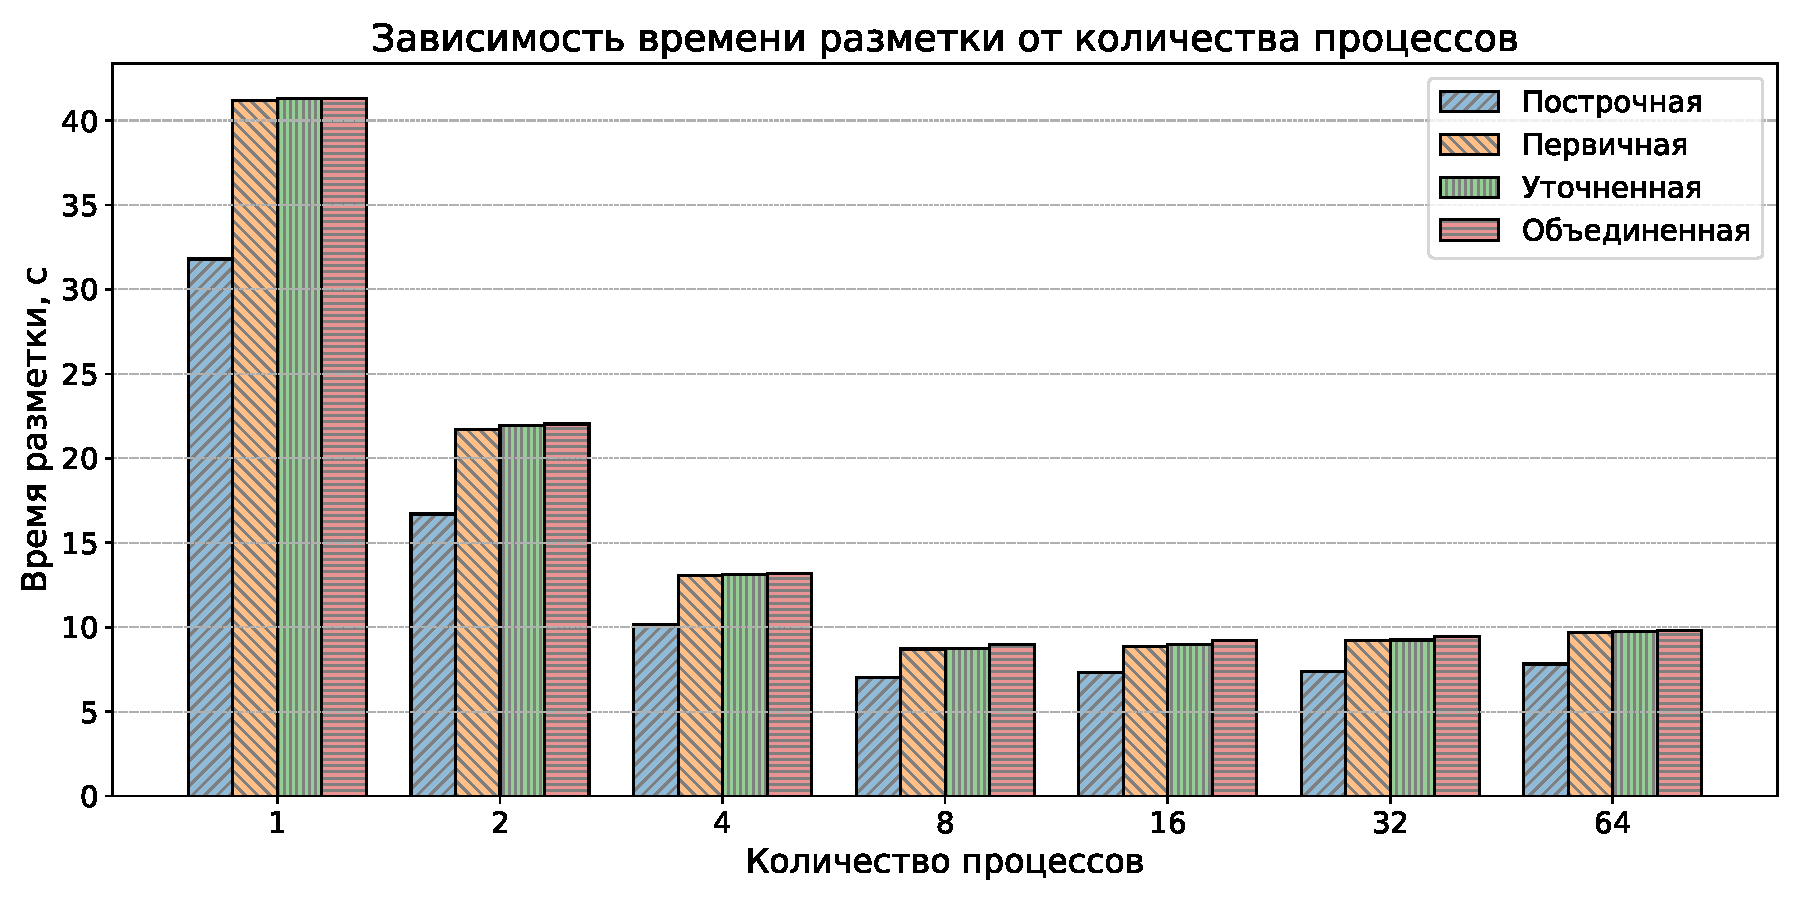
\includegraphics[width=0.9\textwidth]{diag/tama_bar.pdf}
    \end{figure}

    \vspace{-0.5cm}
    \tiny
    \begin{center}
        \begin{tabular}{|r|r|r|r|r|}
            \hline
            \textbf{Количество процессов} & \textbf{Построчн.}, c & \textbf{Первичн.}, c & \textbf{Уточн.}, c & \textbf{Объед., c} \\ \hline
            1 & 31.80 & 41.21 & 41.29 & 41.31 \\ \hline
            2 & 16.70 & 21.72 & 21.96 & 22.03 \\ \hline
            4 & 10.16 & 13.05 & 13.11 & 13.19 \\ \hline
            8 & 7.03 & 8.71 & 8.72 & 8.96 \\ \hline
            16 & 7.29 & 8.83 & 8.96 & 9.23 \\ \hline
            32 & 7.40 & 9.23 & 9.24 & 9.47 \\ \hline
            64 & 7.82 & 9.67 & 9.73 & 9.79 \\ \hline
        \end{tabular}
    \end{center}
\end{frame}

\begin{frame}
    \frametitle{Зависимость максимального объема используемой памяти от количества рабочих процессов}
    % Закончили основную часть, пришли к исследованию (10-11, минимум 2 слайда). Нельзя описать исследование и повторить заголовок. Только конкретика исследования. Если удастся создать что-то, что сравнимо с уже существующим — можно сравнить и по сложности, и по времени.
    \begin{figure}[H]
        \centering
        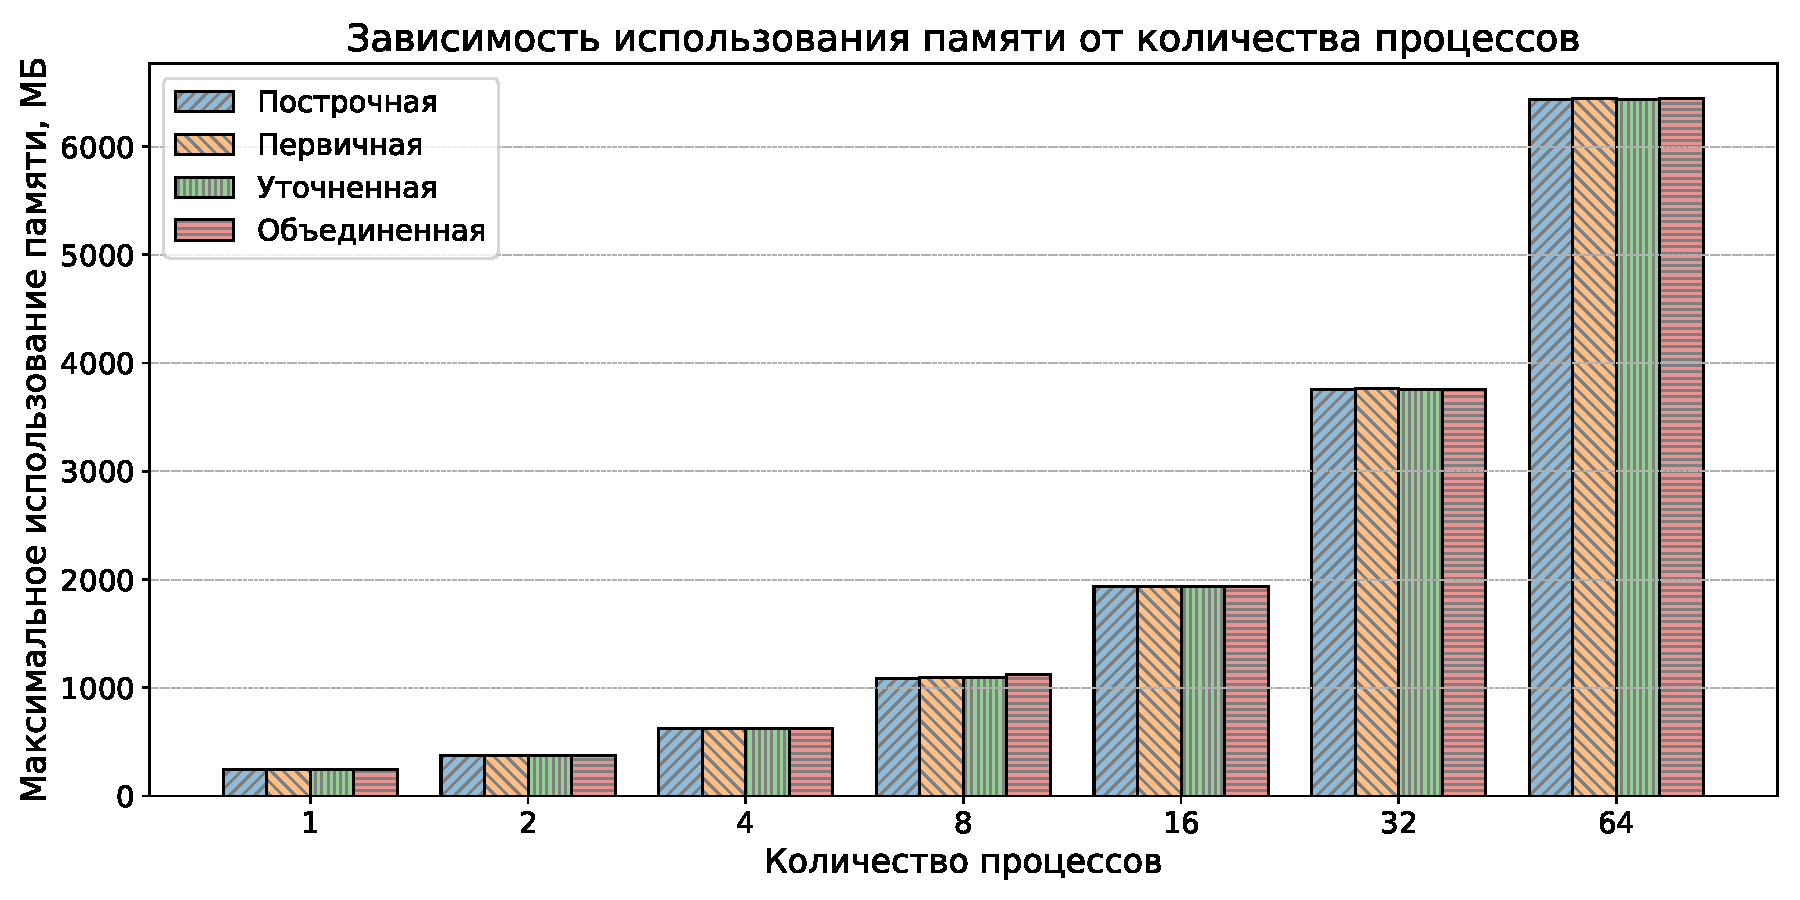
\includegraphics[width=0.9\textwidth]{diag/pama_bar.pdf}
    \end{figure}

    \vspace{-0.5cm}
    \tiny
    \begin{center}
        \begin{tabular}{|r|r|r|r|r|}
            \hline
            \textbf{Количество процессов} & \textbf{Построчн.}, МБ & \textbf{Первичн.}, МБ & \textbf{Уточн.}, МБ & \textbf{Объед., МБ} \\ \hline
            1 & 247.39 & 246.58 & 246.56 & 245.09 \\ \hline
            2 & 374.05 & 373.12 & 373.26 & 373.16 \\ \hline
            4 & 627.94 & 625.74 & 627.79 & 627.11 \\ \hline
            8 & 1085.41 & 1096.95 & 1098.18 & 1122.85 \\ \hline
            16 & 1933.34 & 1934.43 & 1932.78 & 1935.12 \\ \hline
            32 & 3757.83 & 3760.95 & 3758.53 & 3758.38 \\ \hline
            64 & 6437.75 & 6444.76 & 6438.00 & 6440.77 \\ \hline
        \end{tabular}
    \end{center}
\end{frame}

\begin{frame}
    \frametitle{Точность и полнота качества работы}

    \begin{table}[H]
        % \centering
        \begin{center}
            \begin{tabular}{|c|c|c|c|c|c|}
                \hline
                \textbf{Класс \textbackslash\ Критерий} & \textbf{Верно} & \textbf{Л-П.} & \textbf{Л-Н.} & Точность & Полнота \\ \hline
                Фон & 73 & 0 & 0 & 1.00 & 1.00 \\ \hline
                Текст & 490 & 15 & 1 & 0.97 & 0.99 \\ \hline
                Схема & 92 & 17 & 41 & 0.84 & 0.69 \\ \hline
                Рисунок & 50 & 54 & 21 & 0.48 & 0.83 \\ \hline
                График & 37 & 10 & 9 & 0.79 & 0.80 \\ \hline
                Таблица & 90 & 0 & 12 & 1.00 & 0.88 \\ \hline
                Листинг & 80 & 4 & 18 & 0.95 & 0.82 \\ \hline
                Не определено & 20 & 0 & 0 & 1.00 & 1.00 \\ \hline
            \end{tabular}
        \end{center}
    \end{table}
\end{frame}

\begin{frame}
    \frametitle{Заключение}

    Цель достигнута: Разработан метод для автоматического выделения составных частей научного текста, использующего только простые эвристики для классификации сегментов документа.

    \vspace{0.2cm}

    Решены все задачи:
    \begin{itemize}
        \item Рассмотрены и сравнены существующие методы сегментации документов;
        \item Формализована постановка задачи;
        \item Разработан описанный метод;
        \item Разработано программное обеспечение, реализующее данный метод;
        \item Проведено исследование скорости разметки и максимального объема используемой памяти в зависимости от количества процессов, участвующих в разметке.
    \end{itemize}
\end{frame}

\begin{frame}
    \frametitle{Дальнейшее развитие}
    \begin{itemize}
        \item Добавление новых правил для учета дополнительных классов таблиц и рисунков в текстах;
        \item Поддержка классификации формул;
        \item Поддержка работы с двухколоночными документами.
    \end{itemize}

    \vfill

    \begin{center}
        \large Внедрение
    \end{center}

    \begin{itemize}
        \item Планируется интеграция разработанного модуля разметки в систему проведения нормоконтроля МГТУ~им.~Н.~Э.~Баумана в осеннем семестре 2025 года.
    \end{itemize}

    % \vfill
    %
    % \begin{center}
    %     \large Публикационная активность
    % \end{center}
    %
    % \begin{itemize}
    %     \item Опубликована статья <<Рунов К.А. Проектирование базы данных для разметки параллельного корпуса технических текстов>> в сборнике материалов <<Инновационные, информационные и коммуникационные технологии: сборник трудов XXI Международной научно-практической конференции>> (РИНЦ).
    % \end{itemize}
\end{frame}

\begin{frame}
    \frametitle{Публикационная активность}
    
    \begin{itemize}
        \item Опубликована статья <<Рунов К.А. Проектирование базы данных для разметки параллельного корпуса технических текстов>> в сборнике трудов XXI Международной научно-практической конференции <<Инновационные, информационные и коммуникационные технологии>> (РИНЦ).
    \end{itemize}
\end{frame}

\end{document}
